\documentclass{article}

\usepackage{microtype}
\usepackage{graphicx}
\usepackage{subfigure}
\usepackage{booktabs}
\usepackage{amsmath}
\usepackage{amssymb}
\usepackage{hyperref}

\newcommand{\theHalgorithm}{\arabic{algorithm}}

\usepackage[accepted]{icml2021}

\icmltitlerunning{Fewer Fruits, Fewer Bites: SARSA vs Q-learning on Snake}

\begin{document}

\twocolumn[
\icmltitle{Fewer Fruits, Fewer Bites:\\SARSA vs Q-learning on Snake under Full and Partial Observability}

\begin{icmlauthorlist}
\icmlauthor{Matteo Polo}{}
\end{icmlauthorlist}

\icmlkeywords{Reinforcement Learning, SARSA, Q-learning, Reward Design, Partial Observability, UniPD}

\vskip 0.3in
]

%\printAffiliationsAndNotice{}

\begin{abstract}
We train a convolutional Q-network to play Snake with SARSA and Q-learning.
By the end of the training, our first implementation ate about 72 fruits per episode, but lost almost all of them in about 6 self-collisions.
We therefore shifted the goal of the project to eating as many fruits as possible \emph{while avoiding self-collisions} as much as possible, and redesigned the reward, the allowed moves and the training loop accordingly.
Compared with the first implementation, self-collisions drop by about 65\% and lost segments by about 75\%, at the cost of about 40\% fewer fruits.
We then compare the two algorithms under full and partial ($5\times5$ window) observability.
With a fixed learning rate the greedy policy is unstable, especially with the window, where it often gets stuck in loops; a cosine learning-rate decay removes most of this instability.
After this fix all four configurations reach about 40 fruits per game in greedy evaluation, and the main remaining difference is in training: with the full board Q-learning takes more risk than SARSA.
\end{abstract}

% ---------------------------------------------------------------------------
\section{Introduction}
\label{sec:intro}

Snake is a small control problem with a delayed, competing objective: eating a fruit makes the snake longer, and a longer snake is harder to steer without biting itself.
Our project had two goals: (i) eat as many fruits as possible, (ii) avoid self-collisions; and one question: how do on-policy SARSA \cite{rummery1994} and off-policy Q-learning \cite{watkins1992} differ on this trade-off when the agent sees the whole board versus only a window around its head?

Most of the work went into \emph{making the agents learn the intended behaviour} rather than into the algorithms themselves.
Each fix exposed a new failure mode, so the paper is organised as a sequence of design decisions (Section~\ref{sec:design}), each motivated by an observed failure.
Our contributions are:
\begin{itemize}
\item a diagnosis of reward hacking in the provided reward and a corrected collision penalty that makes self-collisions strictly unprofitable (Section~\ref{sec:hacking});
\item a set of minimal changes (action masks, step cost, per-episode reset, potential-based shaping) that turn a degenerate policy into one that grows the snake (Sections~\ref{sec:collapse}--\ref{sec:shaping});
\item evidence that the instability of the greedy policy between checkpoints comes from the fixed learning rate, and that a cosine decay removes most of it (Section~\ref{sec:lr});
\item a controlled $2\times2$ comparison (algorithm $\times$ observability) in which the two scripts differ \emph{only} in the TD target and the two environments differ \emph{only} in the observation (Section~\ref{sec:results}).
\end{itemize}

% ---------------------------------------------------------------------------
\section{Setup}
\label{sec:setup}

\subsection{Environment}
Each board is a $10\times10$ grid surrounded by walls, i.e.\ 64 free cells (Figure \ref{fig:map}).
At every step the agent picks one of four moves.
Three facts about the setup matter for everything that follows:
\begin{itemize}
\item a \textbf{self-collision does not end the game}: the tail is cut from the bitten segment onwards and the snake keeps moving;
\item a \textbf{wall hit does not end the game} either: the head stays still while the tail retracts by one cell;
\item 32 boards are simulated in parallel, and an \emph{episode} is a window of 500 steps.
\end{itemize}


\begin{figure}[htp]
    \centering
    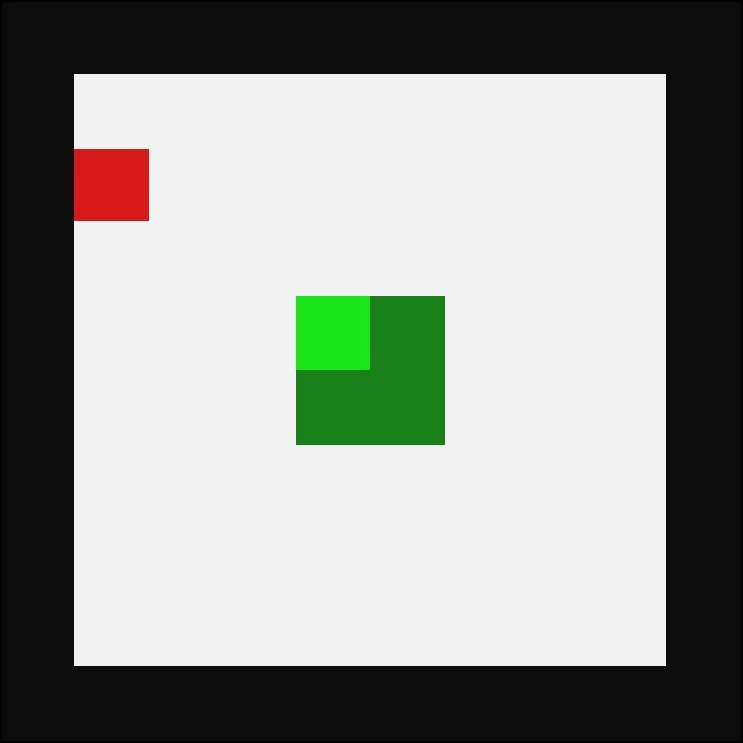
\includegraphics[width=0.5\columnwidth]{figures/snake_map.jpg}
    \caption{A $10\times10$ board: walls (black), head (light green), body (dark green), fruit (red).}
    \label{fig:map}
\end{figure}

Since nothing is terminal, the end of an episode is a time-limit truncation, and we keep bootstrapping on the last transition \cite{pardo2018}.

\subsection{State representation}
The board is one-hot encoded into four channels (empty, fruit, body, head); walls are the all-zero vector.
\begin{itemize}
\item \textbf{Fully observable (FO):} the whole $10\times10\times4$ board.
\item \textbf{Partially observable (PO):} a $(2m+1)\times(2m+1)\times4$ window centred on the head, with $m=2$ ($5\times5$). Cells outside the board are padded as walls.
\end{itemize}
The two environment files are identical except for this observation: with the same seed and actions they produce the same boards and rewards (checked over 3000 steps on 32 boards).
We chose $m=2$ because it always contains the cells the agent can reach in two moves, so immediate dangers are visible, while the fruit is usually not.

\subsection{Original implementation}
Our first implementation, which we call the \emph{original} agents, used the environment reward as given (Table~\ref{tab:reward}), no action masks (reversals and wall hits allowed), games that continued across episodes, and no shaping. Its two scripts also used different $\varepsilon$ schedules (SARSA $0.2\to0.02$, Q-learning constant $0.15$). Network, heuristic, 32 boards and 200 episodes of 500 steps are the same as in the modified agents. Section~\ref{sec:design} motivates every change, and Section~\ref{sec:results} measures the result.

\subsection{Network and exploration}
Both algorithms share the same Q-network: two $3\times3$ convolutions (32 and 64 filters, \emph{same} padding), a dense layer of 128 units and a linear output with 4 Q-values.
In PO only the input size changes.
We train online with Adam, with a learning rate that decays from $10^{-3}$ to $10^{-4}$ along a cosine (Section~\ref{sec:lr}), MSE on the TD error, one gradient step per environment step on the 32 transitions, $\gamma=0.95$, for 200 episodes.

Exploration is $\varepsilon$-greedy with $\varepsilon$ decaying linearly from $0.2$ to $0.02$, but the exploratory move is not uniform: it comes from a rule-based heuristic that never reverses, avoids walls and body, and moves toward the fruit (ties broken at random).
Uniform exploration on a crowded board mostly produces collisions, which would drown the learning signal.
In PO the heuristic only sees the $5\times5$ window: if the fruit is outside, it picks a random safe move.

% ---------------------------------------------------------------------------
\section{Algorithms}
\label{sec:algo}

The two methods differ only in the TD target.
Let $\mathcal{A}(s)$ be the set of \emph{allowed} actions in $s$ (no wall, no reversal; Section~\ref{sec:collapse}). Then
\begin{align}
y^{\textsc{sarsa}} &= r + \gamma\, Q(s',a'), \quad a' \sim \pi_\varepsilon(\cdot \mid s'), \label{eq:sarsa}\\
y^{\textsc{ql}} &= r + \gamma \max_{a \in \mathcal{A}(s')} Q(s',a). \label{eq:ql}
\end{align}
In both cases $a'$ is chosen only among the allowed actions $\mathcal{A}(s')$. SARSA evaluates the behaviour policy, exploration included. Q-learning evaluates the greedy policy.
The $\max$ in \eqref{eq:ql} is restricted to $\mathcal{A}(s')$; otherwise the target would bootstrap on moves the agent can never take.
The training loop is summarised in Algorithm~\ref{alg:train}.
%the two scripts are generated from the same code, and a \texttt{diff} confirms that only the target computation and file names differ.

\begin{algorithm}[tb]
   \caption{Training loop (shared by SARSA and Q-learning)}
   \label{alg:train}
\begin{algorithmic}
   \FOR{episode $=1$ {\bfseries to} $200$}
   \STATE Reset the 32 boards; set $\varepsilon$ (linear decay)
   \STATE Choose $a$: greedy over $\mathcal{A}(s)$, heuristic w.p.\ $\varepsilon$
   \FOR{$t=1$ {\bfseries to} $500$}
   \STATE Execute $a$; observe environment reward and $s'$
   \STATE $r \leftarrow$ reward \eqref{eq:collision} $+$ step cost $+$ $F$ \eqref{eq:shaping}
   \STATE Choose $a'$ in $s'$ as above
   \STATE $y \leftarrow$ \eqref{eq:sarsa} (SARSA) or \eqref{eq:ql} (Q-learning)
   \STATE One Adam step on $\frac{1}{32}\sum_{b}\big(y_b - Q(s_b,a_b)\big)^2$
   \STATE $s \leftarrow s'$, $a \leftarrow a'$
   \ENDFOR
   \STATE Every 10 episodes: greedy evaluation on 20 new games
   \ENDFOR
\end{algorithmic}
\end{algorithm}

% ---------------------------------------------------------------------------
\section{Design decisions}
\label{sec:design}

Table~\ref{tab:reward} summarises the final reward. Each subsection explains one change through the failure that motivated it. Sections~\ref{sec:hacking}--\ref{sec:shaping} were tested with SARSA in FO on short 60-episode runs, and their numbers come from those runs; the learning-rate decay (Section~\ref{sec:lr}) was tested on all four configurations with 200 episodes.

\begin{table}[t]
\caption{Reward per step. $k$ = segments lost in a self-collision, $d$ = Manhattan distance head--fruit.}
\label{tab:reward}
\vskip 0.1in
\begin{center}
\begin{small}
\begin{tabular}{lcc}
\toprule
Event & Original & Modified \\
\midrule
Fruit eaten        & $+0.5$      & $+0.5$ \\
Self-collision     & $-0.1\,k$   & $-(0.5+0.5\,k)$ \\
Wall hit           & $-0.3$      & masked \\
Any step           & $0$         & $-0.01$ \\
Shaping            & --          & $\gamma\Phi(s')-\Phi(s)$ \\
\bottomrule
\end{tabular}
\end{small}
\end{center}
\vskip -0.15in
\end{table}

\subsection{Reward hacking: ``eat, then bite''}
\label{sec:hacking}
With the provided reward the original agents reached a stable, positive return (about $+29$ per episode), yet the snake stayed short: per episode they ate about 72 fruits and lost about 71 segments in about 6 self-collisions (Figure~\ref{fig:origmod}).
The reason is arithmetic. A segment is worth $+0.5$ when gained but costs only $-0.1$ when lost, so the cycle ``eat $k$ fruits, then cut $k$ segments'' yields
\begin{equation}
0.5k - 0.1k = +0.4k > 0 .
\end{equation}
Discounting makes it worse, because the fruit comes before the penalty, and a short snake also reaches fruits faster.
This is specification gaming \cite{amodei2016,krakovna2020}: the agent maximises the reward it is given, and that reward disagrees with goal (ii).
Potential-based shaping cannot fix this, since by construction it preserves the optimal policy \cite{ng1999}; the reward itself has to change.
We replace the collision penalty with
\begin{equation}
r_{\text{self}}(k) = -(0.5 + 0.5\,k).
\label{eq:collision}
\end{equation}
The proportional part gives back exactly what the lost segments were worth, so the cycle becomes neutral; the fixed part makes it strictly negative, $0.5k-(0.5+0.5k)=-0.5$.
When a collision is unavoidable, the dependence on $k$ still prefers biting close to the tail.

We also found that our original implementation counted self-collisions from the reward value, so a collision costing exactly 3 segments ($3\times(-0.1)=-0.3$) was mistaken for a wall hit: 12.6\% of collisions in a test run.
All our metrics are computed from the board state instead, so \emph{the original collision counts are underestimates}.

\subsection{Passive collapse: action masks and step cost}
\label{sec:collapse}
With \eqref{eq:collision} alone, the agent stopped eating: a snake of length 1 oscillated between two cells for the whole episode, with return 0.
At length 1 a reversal is free; after one fruit the same reversal bites the neck, worth $0.5-1.0=-0.5$. Not eating (value 0) is therefore a local optimum of the learning dynamics, not of the task.
Two changes remove it:
\begin{itemize}
\item \textbf{Reversal mask.} The move onto the neck is impossible in real Snake, so we set its Q-value to $-\infty$ before the $\arg\max$. At length 1 we mask the opposite of the last direction.
\item \textbf{Step cost} $-0.01$. Wandering forever is now worth $-0.01/(1-\gamma)=-0.2$ instead of 0.
\end{itemize}
Bites on the rest of the body are \emph{not} masked: avoiding traps is what the network must learn.

\subsection{Wall loops}
\label{sec:walls}
After the previous fix the snake grew (mean length from 3.5 to 35.6), but the training return \emph{decreased}. Splitting the return into its terms showed why: wall hits rose from about 5 to 45 per episode.
A wall hit leaves the state almost unchanged (the head does not move), so a greedy choice of ``wall'' is repeated at the next step; at length 1 the loop is infinite.
We mask wall moves too \cite{huang2022}, so that $\mathcal{A}(s)$ excludes walls and reversals, consistently with the heuristic.
Wall hits dropped to 0. At steady state the return is $\approx -5 - 0.5\cdot(\text{collisions})$, because fruits and lost segments cancel; the training return is therefore a poor progress measure, and we report task metrics instead.

\subsection{Distribution shift: per-episode reset and greedy evaluation}
\label{sec:reset}
In our original implementation the games continued across episodes, so after a few episodes the network almost only sees long snakes.
A separate greedy evaluation ($\varepsilon=0$, 20 new games of 500 steps, fixed seed) revealed the problem: the network that ate about 30 fruits per episode in training mostly ate 0--1 fruits in new games, looping with a short snake.
Resetting the boards at every episode keeps the start of the game in the training data. Greedy evaluation went from 9 to 23 fruits at episode 59 of the same configuration, and the per-episode return became comparable across episodes.
Because averages hide bimodal outcomes, the evaluation also counts \emph{stuck} games: games with no fruit in the last 100 steps, typically a loop.

\subsection{Potential-based shaping toward the fruit}
\label{sec:shaping}
The greedy policy still entered long cycles (period 12--20) after a few fruits, while in training it ate steadily.
In training a few heuristic moves per game (at $\varepsilon\approx0.02$, about 10) are enough to break a cycle, so the network can leave ``go to the fruit'' to the exploration.
For SARSA this is structural, since \eqref{eq:sarsa} values the policy \emph{with} its exploration.
We add
\begin{equation}
F(s,s') = \gamma\Phi(s')-\Phi(s), \qquad \Phi(s) = C\,(D_{\max}-d(s)),
\label{eq:shaping}
\end{equation}
with $C=0.02$ and $D_{\max}=14$, the largest distance on the board.
$F$ leaves the optimal policy unchanged \cite{ng1999}, and $\Phi\ge0$ is deliberate: along a cycle returning to the same state the shaping sums to $(\gamma-1)\sum\Phi\le0$, so going around in circles costs.
Training metrics did not change, but the mean greedy evaluation over checkpoints 10--59 went from 13.5 to 23.9 fruits.
In PO, $\Phi$ uses the true fruit position even when the fruit is not visible. This is legitimate, because the reward belongs to the environment and not to the observation, but the reward then carries indirect information about where the fruit is.

\subsection{Instability: learning-rate decay}
\label{sec:lr}
With all the previous changes and a fixed learning rate of $10^{-3}$, the 200-episode runs still alternated good and broken checkpoints a few episodes apart, up to the end of training (grey lines in Figure~\ref{fig:lr}), while the training curves stayed smooth.
Across the checkpoints from episode 100 on, greedy fruits had a standard deviation of about 10, and in PO 4 of 11 checkpoints ate fewer than 10 fruits, with most games stuck (Table~\ref{tab:lr}).
Updates are online on correlated transitions, and with a constant step size even late updates can flip the $\arg\max$ in many states at once.
We therefore let the learning rate decay from $10^{-3}$ to $10^{-4}$ along a cosine over the $10^5$ updates of training: early learning is almost unchanged, while late updates are small.
From episode 110 on, no checkpoint is broken in any configuration (Figure~\ref{fig:lr}), and stuck games drop from 7--13 to 1--5 of 20 (Table~\ref{tab:lr}).
The only broken checkpoint left is SARSA FO at episode 100, when the learning rate is still about $5\cdot10^{-4}$.
The effect is largest in PO, where greedy fruits more than double.

\begin{table}[t]
\caption{Greedy evaluation with a fixed vs decaying learning rate, over the checkpoints from episode 100 on (11 checkpoints, 20 games each). Std = standard deviation across checkpoints; broken = checkpoints with fewer than 10 fruits.}
\label{tab:lr}
\vskip 0.1in
\begin{center}
\begin{small}
\setlength{\tabcolsep}{3pt}
\begin{tabular}{lcccc}
\toprule
 & Fruit & Std & Broken & Stuck \\
\midrule
SARSA, FO    & 29.7 $\to$ 34.5 & 10.1 $\to$ 10.4 & 1 $\to$ 1 & 7.0 $\to$ 5.3 \\
Q-learn., FO & 27.2 $\to$ 41.9 & 10.1 $\to$ 4.6  & 1 $\to$ 0 & 8.4 $\to$ 1.3 \\
SARSA, PO    & 17.5 $\to$ 39.2 & 11.2 $\to$ 3.3  & 4 $\to$ 0 & 13.1 $\to$ 1.4 \\
Q-learn., PO & 16.1 $\to$ 37.6 & 12.2 $\to$ 7.1  & 4 $\to$ 0 & 13.4 $\to$ 2.5 \\
\bottomrule
\end{tabular}
\end{small}
\end{center}
\vskip -0.15in
\end{table}

\begin{figure}[t]
\begin{center}
\centerline{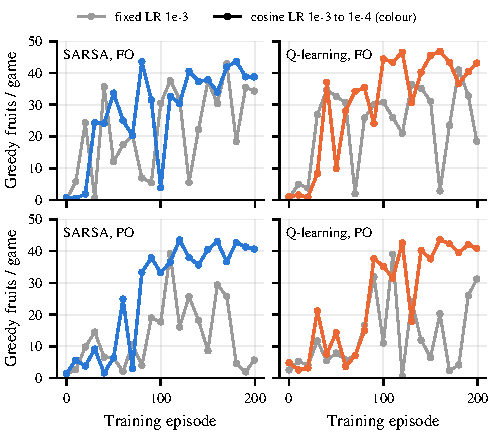
\includegraphics[width=\columnwidth]{figures/lr_fixed_vs_cosine.pdf}}
\caption{Greedy evaluation (fruits per game, 20 games) at every checkpoint, with a fixed learning rate (grey) and a cosine decay (colour), one panel per configuration. With the decay the policy stops oscillating in the second half of training.}
\label{fig:lr}
\end{center}
\vskip -0.3in
\end{figure}

% ---------------------------------------------------------------------------
\section{Results}
\label{sec:results}

All runs use the final configuration (learning-rate decay included), 200 episodes and one seed. Training metrics are averaged over the last 50 episodes. Greedy metrics are averaged over the checkpoints from episode 100 on.

\begin{figure*}[t]
\begin{center}
\centerline{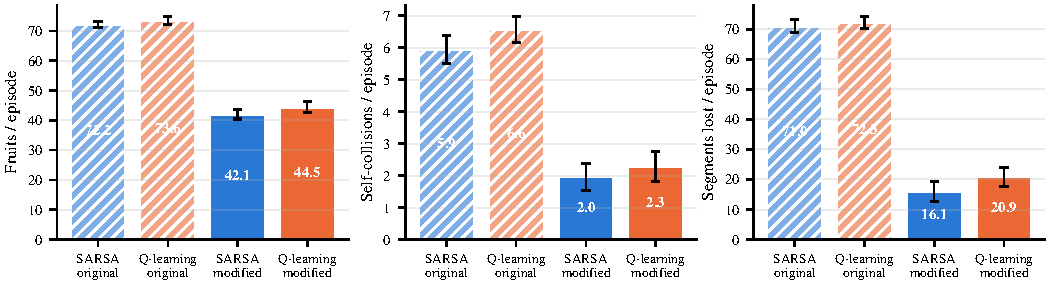
\includegraphics[width=\textwidth]{figures/orig_vs_mod.pdf}}
\caption{Original vs modified agents (FO), mean $\pm$ std over the last 50 training episodes. Hatched: original scripts. The modified agents eat about 40\% fewer fruits, but make about 65\% fewer self-collisions and lose about 75\% fewer segments. The original collision counts are underestimates (Section~\ref{sec:hacking}).}
\label{fig:origmod}
\end{center}
\vskip -0.3in
\end{figure*}

\subsection{Original vs modified}
Figure~\ref{fig:origmod} compares the original scripts with the modified ones.
Fruits drop from 72--74 to 44--45 per episode, self-collisions from 5.9--6.6 to 1.6--2.9, and lost segments from 71--72 to 14--22.
The original agents lost almost every segment they gained; ours keep them, and the mean length grows to 20--22.
Measured as fruits per self-collision, efficiency rises from about 12 to 16 (Q-learning) and 28 (SARSA).

The comparison is not perfectly controlled: the original agents do not reset the games between episodes, so an episode measures a different slice of play, and they use different $\varepsilon$ schedules (Section~\ref{sec:setup}).
The fruit gap is therefore not only a cost of caution. The effect on collisions and lost segments, however, is large and consistent in both algorithms.

\begin{figure}[t]
\begin{center}
\centerline{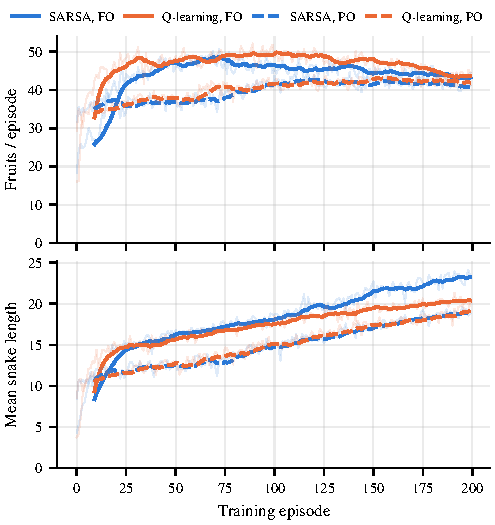
\includegraphics[width=\columnwidth]{figures/training_growth.pdf}}
\caption{Training: fruits per episode (top) and mean snake length (bottom), moving average over 10 episodes. Colour: algorithm; solid: fully observable (FO); dashed: partially observable (PO, $5\times5$ window).}
\label{fig:growth}
\end{center}
\vskip -0.3in
\end{figure}

\begin{figure}[t]
\begin{center}
\centerline{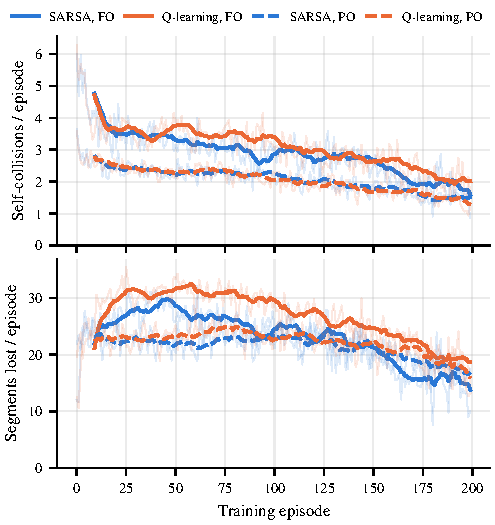
\includegraphics[width=\columnwidth]{figures/training_safety.pdf}}
\caption{Training: self-collisions (top) and segments lost (bottom) per episode, same encoding as Figure~\ref{fig:growth}. Both decrease steadily in the second half of training.}
\label{fig:safety}
\end{center}
\vskip -0.3in
\end{figure}

\begin{table}[t]
\caption{$2\times2$ comparison. Training: mean of the last 50 episodes. Greedy: mean over checkpoints $\ge 100$ (20 games each); Bite = self-collisions, Lost = segments lost, Len.\ = mean snake length (per episode); stuck = games with no fruit in the last 100 steps.}
\label{tab:2x2}
\vskip 0.1in
\begin{center}
\begin{small}
\setlength{\tabcolsep}{3.5pt}
\begin{tabular}{lcccccc}
\toprule
 & \multicolumn{4}{c}{Training} & \multicolumn{2}{c}{Greedy} \\
\cmidrule(lr){2-5}\cmidrule(lr){6-7}
 & Fruit & Bite & Lost & Len. & Fruit & Stuck \\
\midrule
SARSA, FO      & 44.0 & 1.55 & 13.7 & 22.5 & 34.5 & 5.3 \\
Q-learn., FO   & 45.2 & 2.88 & 22.4 & 20.0 & 41.9 & 1.3 \\
SARSA, PO      & 41.5 & 1.71 & 19.1 & 18.3 & 39.2 & 1.4 \\
Q-learn., PO   & 42.4 & 1.62 & 20.1 & 18.3 & 37.6 & 2.5 \\
\bottomrule
\end{tabular}
\end{small}
\end{center}
\vskip -0.15in
\end{table}

\subsection{SARSA vs Q-learning, FO vs PO}
Table~\ref{tab:2x2} and Figures~\ref{fig:growth}--\ref{fig:eval} report the $2\times2$ design.

\textbf{Fruits vs length.} In FO, fruits per episode peak at about 47--50 between episodes 25 and 125 and then decrease to 44--45 (Figure~\ref{fig:growth}), while the snake keeps growing and collisions keep falling (Figure~\ref{fig:safety}). The agent trades fruits for safety: a longer body needs longer, safer paths to the fruit. The numbers in Table~\ref{tab:2x2} are taken at the end of training, after this trade-off.

\textbf{Algorithm (FO).} Q-learning eats about as much as SARSA (45.2 vs 44.0) but bites almost twice as often (2.88 vs 1.55) and loses about 60\% more segments (22.4 vs 13.7).
This is consistent with the textbook difference \cite{sutton2018}: SARSA learns the value of the exploring policy, so it prices in the occasional wrong move near the body and keeps a safer margin, while Q-learning values the greedy path and takes tighter routes.
In greedy evaluation Q-learning is ahead (41.9 vs 34.5), but the SARSA mean is pulled down by a single broken checkpoint (episode 100); from episode 110 on SARSA averages 37.6.

\textbf{Observability.} During training PO costs little: about 6\% fewer fruits and a shorter snake (18.3 vs 20--22.5). PO collisions are lower partly \emph{because} the snake is shorter.
In greedy evaluation there is no clear gap: 38--39 fruits in PO vs 35--42 in FO, with 1--3 of 20 games stuck.
With a $5\times5$ window, many different states produce the same observation whenever the fruit is out of view (perceptual aliasing \cite{kaelbling1998}), and a deterministic memoryless policy can then repeat the same cycle forever \cite{singh1994}.
With a fixed learning rate we attributed the many stuck PO games to this effect, but the decay removes most of them (Table~\ref{tab:lr}): in our setting the loops came mainly from unstable updates.
Two caveats remain: the shaping term uses the true fruit position (Section~\ref{sec:shaping}), so the reward partly makes up for what the window hides, and the board is small, so the fruit is often within a few moves.
Under PO the two algorithms are indistinguishable.

\begin{figure}[t]
\begin{center}
\centerline{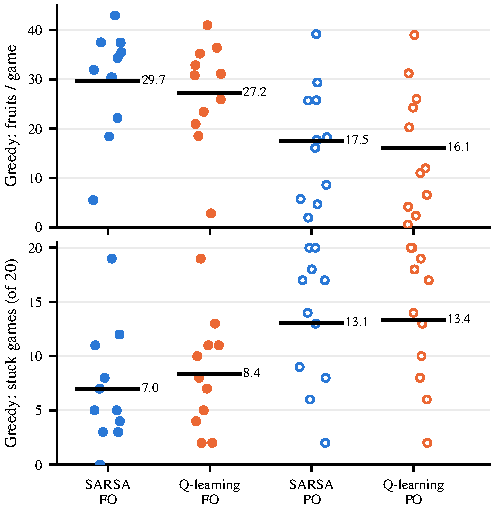
\includegraphics[width=\columnwidth]{figures/eval_2x2.pdf}}
\caption{Greedy evaluation ($\varepsilon=0$, 20 new games, fixed seed) of every checkpoint from episode 100 on: one dot per checkpoint, black line = mean. Top: fruits per game; bottom: stuck games. Filled: FO; hollow: PO. The outlier at about 4 fruits is the SARSA FO checkpoint at episode 100.}
\label{fig:eval}
\end{center}
\vskip -0.3in
\end{figure}

% ---------------------------------------------------------------------------
\section{Discussion and limitations}
\label{sec:discussion}

\textbf{Training metrics can mislead.} Each failure in Section~\ref{sec:design} was invisible in at least one standard curve: reward hacking had a rising return, the wall loops had a falling return with improving behaviour, and the distribution shift and the cycles only appeared in greedy evaluation on new games. Logging task metrics (length, lost segments, stuck games) and watching the games was essential.

\textbf{Behaviour vs greedy policy.} With a smart exploration heuristic, part of the competence lives in the exploration, not in the network. Before the learning-rate decay this showed up as a large gap between training and greedy performance, especially in PO; after it, greedy games reach about 40 fruits per 500 steps, close to the 41--45 per episode in training.

\textbf{Instability.} With a fixed learning rate the greedy policy alternated good and broken checkpoints while training curves stayed smooth. Experience replay and a target network \cite{mnih2015} are the standard remedies; we kept the plain online algorithms, to compare SARSA and Q-learning in their textbook form, and a decaying step size was enough. A single, slow evaluation can therefore mislead: one checkpoint of a fixed-rate run can look much better or much worse than the agent really is.

\textbf{Limitations.}
\begin{itemize}
\item There is one seed per configuration, so the small SARSA vs Q-learning differences are suggestive, not conclusive.
\item The original runs undercount collisions and use different $\varepsilon$ schedules.
\item In PO the shaping term uses the true fruit position.
\item We tried a single learning-rate schedule ($10^{-3}\to10^{-4}$, cosine), with no comparison to other schedules.
\end{itemize}
Natural next steps are several seeds with confidence intervals, PO without fruit information in the reward to measure aliasing on its own, a larger board where the window hides more, and giving the PO agent memory (frame stacking or a recurrent network \cite{hausknecht2015}).

% ---------------------------------------------------------------------------
\section{Conclusion}
\label{sec:conclusion}

The provided reward taught both algorithms to eat and bite. Making self-collisions strictly unprofitable, masking moves the game forbids, resetting games and shaping toward the fruit produced agents that eat about 40\% fewer fruits but bite about 65\% less and keep their length.
SARSA is the more cautious learner under full observability, as theory predicts.
The instability of the greedy policy, which we first attributed to partial observability, came mainly from the fixed learning rate: with a cosine decay all four configurations reach about 40 fruits per game, and a $5\times5$ window costs little on a $10\times10$ board when the reward still points to the fruit.

\bibliography{main}
\bibliographystyle{icml2021}

\end{document}
